\documentclass[a4paper]{article}

%% Language and font encodings
\usepackage[english]{babel}
\usepackage[utf8x]{inputenc}
\usepackage[T1]{fontenc}
\usepackage[]{algorithm2e}

%% Sets page size and margins
\usepackage[a4paper,top=3cm,bottom=2cm,left=3cm,right=3cm,marginparwidth=1.75cm]{geometry}

%% Useful packages
\usepackage{amsmath}
%% argmin command
\DeclareMathOperator*{\argmin}{arg\,min}
\usepackage{graphicx}
\usepackage{url}
\author{Tobias Mathony}
\title{Fachpraktikum Algorithms on OpenStreetMap Data: eMaps}
\date{\today}
\begin{document}
\maketitle
\begin{abstract}
Electrically-powered vehicles, such as e-Bikes or e-Cars, play an important role in today's fight against climate change.
Contrary to traditional vehicles, such as cars running on gasoline, electrical vehicles have unique characteristics like a limited cruising range, and long recharge times.
To ensure that such vehicles never run out of power, adaptions to navigation and route planners are required.
This project explains the implementation of a route planner that considers the limited cruising range of electric vehicles, as well as the availability of charging stations in the road network, based on OpenStreetMap data. 
\end{abstract}
\section{Introduction}
Climate change and its consequences heavily impacted the engineering of means of transport.
As a result, vehicles powered by electric batteries emerged, such as electrically-powered cars, bikes or scooters.
By using regenerative energy sources, electrically-powered vehicles have the potential to significantly reduce the dependency of fossil fuel reserves \cite{Artmeier2010}.
Furthermore, electric vehicles emit no emissions and are therefore more eco-friendly than vehicles running on gasoline.
However, electric vehicles have characteristics that currently hinder its wide-spread adaption, i.e. (i) limited cruising range, and (ii) long recharge times \cite{Artmeier2010}.
Especially the limited cruising range requires an adaption of existing navigation and routing systems.
We need to determine routes for electric vehicles considering the availability of charging stations and the range of electric vehicles to avoid running out of power.\par\medskip
Using OpenStreetMap\footnote{\url{https://www.openstreetmap.org}} data, we demonstrate the implementation of a route planner that considers the range of an electric vehicle and the availability of charging stations. 
\section{OpenStreetMap}
This project is implemented on OpenStreetMap data.
OpenStreetMap (OSM) is a community-driven open-source project that provides user-generated map data \cite{Haklay2008}.
Besides that, also further geographical information like charging stations, bars, clubs or restaurants are available.
OpenStreetMap data is available in different formats with parsers for the most popular programming languages.\par\medskip
\section{Implementation}
This section outlines the architecture of the application, the used technologies and the main features of the implementation.
\begin{figure}
    \centering
    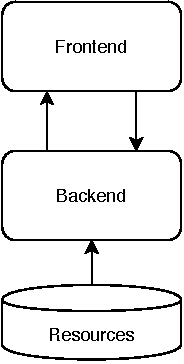
\includegraphics[scale=1]{figures/arch}
    \caption{Conceptual overview of the application}
    \label{fig:arch}
\end{figure}
\subsection{Architecture and Technologies}
For the architecture of the application, the common \textbf{Model-View-Controller} paradigm was used for a strict separation of functionality and an increased re-usability of the components as depicted in Figure \ref{fig:arch}.\par\medskip
The \textbf{Resources} represent the raw OpenStreetMap data which was provided in the \textit{Protocolbuffer Binary Format (PBF)}\footnote{\url{https://wiki.openstreetmap.org/wiki/PBF_Format}}.\par\medskip
The \textbf{Backend} provides the core functionality and implements algorithms on the OpenStreetMap data.
It is implemented as Web Server in \textit{Rust}\footnote{\url{https://www.rust-lang.org}}.
The core functionality of the Backend includes (i) a parser to map the OpenStreetMap data to a \textit{Domain Object Model} (DOM) representation in Rust,
(ii) a shortest path algorithm, and (iii) an \textit{Application Programming Interface} (API) to expose the functionality for access from the Frontend.\par\medskip
The \textbf{Frontend} is built using the \textit{React}\footnote{\url{https://reactjs.org}} Web Framework and \textit{Leaflet}\footnote{\url{https://leafletjs.com}}. Leaflet is an open-source JavaScript library for interactive maps based on OpenStreetMap.
Leaflet is used to provide a user-friendly map and allows to e.g. set markers or draw routes.
Figure \ref{fig:base_ui} displays the Frontend in its initial state.
The Frontend interacts with the Backend via \textit{HTTP} requests.
\begin{figure}[h]
    \centering
    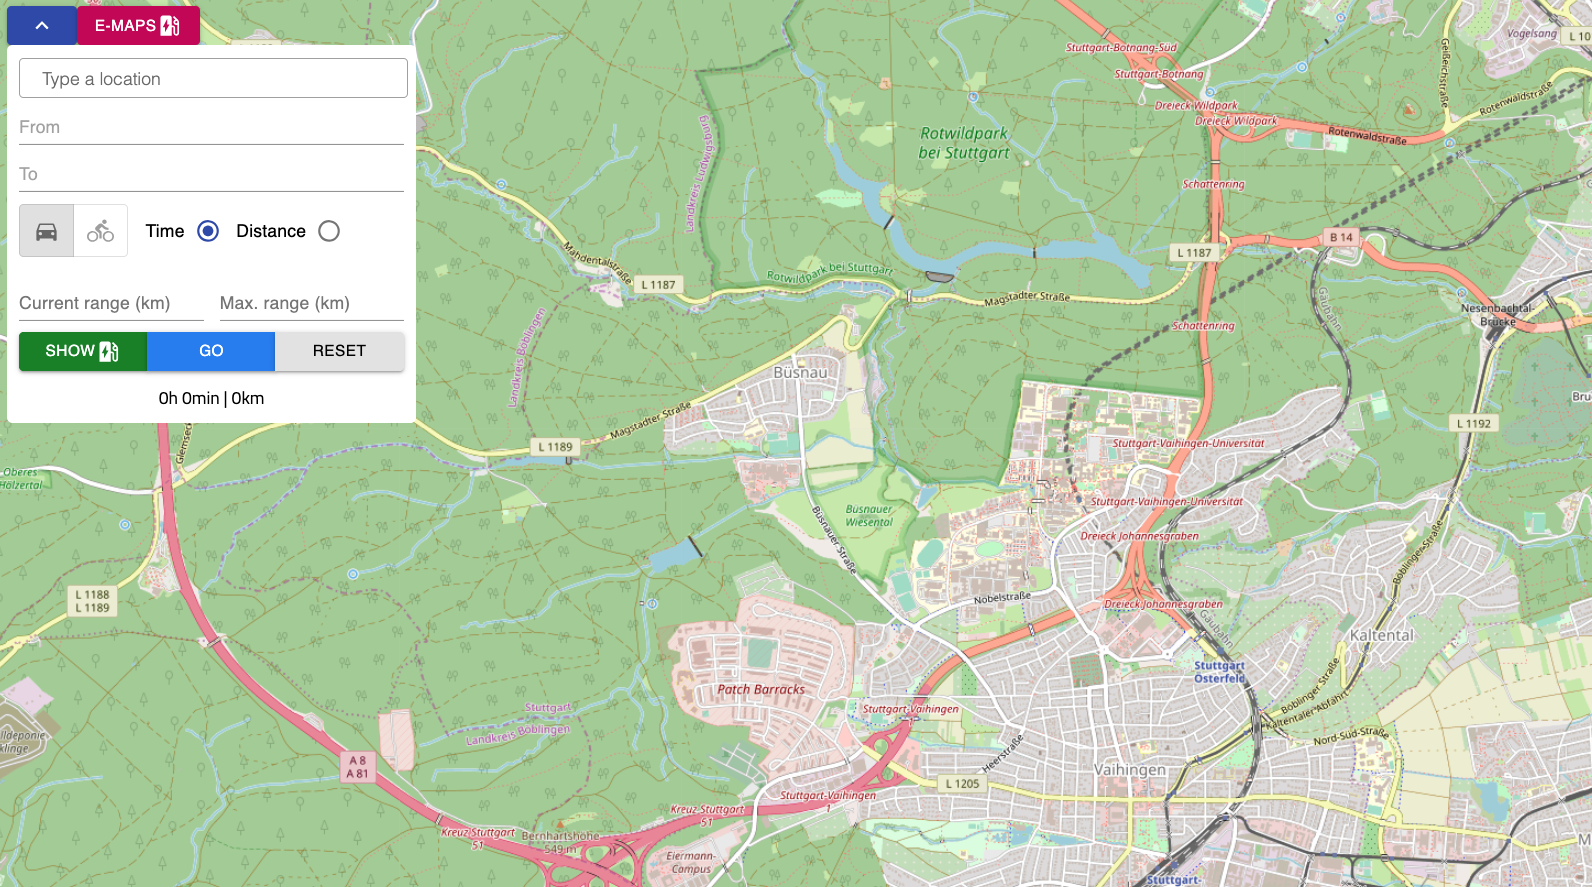
\includegraphics[scale=0.25]{figures/base_ui}
    \caption{Screenshot of the Frontend}
    \label{fig:base_ui}
\end{figure}
\subsection{Graph}
The Backend parses the graph data from OpenStreetMap in the PBF format.
This allows to map the graph data from a PBF file, e.g. the road network graph of Germany, to a DOM representation in Rust.
However, only necessary data is parsed from the PBF file for performance and efficiency reasons.
We focus on \textit{ways}, \textit{nodes}, and \textit{amenities} in OpenStreetMap. A node in OpenStreetMap is a single geographical data point with latitude and longitude. A way is a combination of multiple nodes building a sequence, e.g. a street.
Amenities are arbitrary geographical POIs, e.g. a restaurant, a bar, or a charging station.
Amenities are stored as Key-Value-Pairs in OpenStreetMap, e.g. $\lbrace amenity: charging\_station \rbrace$.
The implementation of this route planner focuses on electric cars and electric bikes, hence we only parse ways where cars and bikes are allowed to drive on.
Furthermore, we parse charging stations from the amenities to be able to consider those later on when calculating a route.\par\medskip
Our graph is structured as follows: $G = \lbrace N, E, O, C, CN \rbrace$ with (i) $N$ being a set of nodes, (ii) $W$ being a set of edges, (iii) $O$ being a offset array, (iv) $C$ being a cell hashmap and $CN$ being a set of nodes that represent a charging station.
The offset array is used to efficiently access the edges of a node. The cell hashmap is used to create a grid layer above the graph to speed up the search of the nearest node in the graph for coordinates.
While creating the graph, every node is hashed into a grid cell using the predecimal digits of latitude and longitude of its coordinates.
When the user requests a shortest path calculation from the Frontend, arbitrary start and target locations may be passed, however since we only parsed ways that are valid for cars and bikes, we may need to locate the nearest node in our graph to the start and target location as passed by the user.
Let us assume we want to locate the nearest node in our graph for a node called $n$.
First, we locate $n$ in the grid by using the predecimal digits of its coordinates. 
Then, we calculate the distance of all nodes in the cell to $n$ and choose the node with the smallest distance to $n$.
Since the nearest node to $n$ may be in another cell, we also check neighboring cells for the nearest neighbor.\\
To extract charging stations from OpenStreetMap, we check for each node if a Key-Value-Pair $\lbrace amenity: charging\_station \rbrace$ exists, i.e. if the node is tagged as charging station in OpenStreetMap.
Besides that, OpenStreetMap data also provides information about the vehicles that can be charged at a charging station.
However, since OpenStreetMap is community-driven and based on user-generated data, not all charging stations contain information about the vehicles that can be charged.
Thus, for charging stations without further information, we just assume that both cars and bikes can be charged.
Hence, a charging station in our graph model contains coordinates, an enum indicating the vehicles that can be charged, and an identifier.
\subsection{Routing}
To route between two nodes in our graph, we use Dijkstra's Shortest Path Algorithm \cite{Dijkstra1959}.
The user is able to select between routing for shortest time or shortest distance, as visible in Figure \ref{fig:input}.
\subsection{Routing for Electric Vehicles}
The main functionality of this project is a route planner that considers the current and maximum range of electric vehicles, as well as charging stations to determine a route where an electric vehicle never runs out of battery.
\begin{figure}[h]
    \centering
    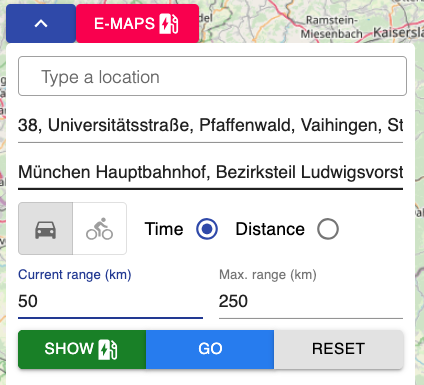
\includegraphics[scale=0.6]{figures/input}
    \caption{Modal for the user to e.g. enter current and maximum range}
    \label{fig:input}
\end{figure}
Figure \ref{fig:input} depicts the modal where the user can enter the current and maximum range of the electric vehicle used for travelling.
Once a start and target location is chosen, the user can submit the request for route planning including the parameters of current and maximum range to the Backend.
Initially, in the Backend, a shortest path calculation is started from start to target.
The pseudo code depicted in Algorithm \ref{alg:route} simplifies the processing of the Backend once receiving such a request.\par\bigskip
\begin{algorithm}[H]
 \KwData{start coordinates, target coordinates, current range, maximum range}
 \KwResult{route}
naive route $\leftarrow$  shortest path(start coordinates, target coordinates)\;
required range $\leftarrow$ route.distance\;
 \While{required range > current range}{
 charging station coordinates $\leftarrow$ find optimal charging station coordinates\;
 route to charging $\leftarrow$ shortest path(start coordinates, charging station coordinates)\;
 route $\leftarrow$ route + route to charging\;
 
 current range $\leftarrow$ maximum range\;
 start coordinates $\leftarrow$ charging station coordinates\;
 
 route to target $\leftarrow$ shortest path(start coordinates, target coordinates)\;
 required range $\leftarrow$ route to target.distance\;
 
  \If{route to target.distance < current range}{
    route $\leftarrow$ route + route to target\;
     \Return{route}
   }
 }
 \Return{naive route}
 \caption{Simplified route calculation}
 \label{alg:route}
\end{algorithm}\par\bigskip
At first, we just calculate a shortest path based on start and target parameters, to check if the current range of our electric vehicle is sufficient.
If it is not sufficient, we reset the route and calculate the optimal charging station coordinates based on the start and target location, as well as the current range and our means of transportation, i.e. car or bike.
This calculation is depicted in Algorithm \ref{alg:charg}. 
For this, we iterate over all charging stations and check as a pre-condition if the current charging station supports our means of transportation.
If this is the case, we calculate the haversine distance to the current charging station from respectively the start and target location.
Then, we check if the charging station is reachable from our start location with the current range, and compare both distances with the global minimum, respectively maximum. 
Our goal is to calculate the charging station which is the farthest away from the start and the closest to the target, i.e. we want to utilize the current range as far as it is possible and get a charging station which is as close to the target location as the current range allows.
Once we determined the charging station coordinates, we calculate the shortest path from the start location to the chosen charging station location.
Then, we set our current range as maximum range, since we assume that we charged our electric vehicle fully.
Then, we set the charging station location as new start and calculate the shortest path again from our new start to the target location.
We update the required range to the distance to the target from the lastly used charging station.
While the required range is still bigger than our current range, we calculate routes between charging stations based on start and target, until we are able to reach the target.
\par\bigskip
\begin{algorithm}[H]
 \KwData{start coordinates, target coordinates, current range, transportation mode}
 \KwResult{chosen charging station}
closest distance from start $\leftarrow$ 0\;
closest distance from goal $\leftarrow$ max\;
 \For{charging station \textbf{in} charging stations}{
 \If{charging station \textbf{contains} transportation mode}{
 temp distance from start $\leftarrow$ distance(start coordinates, charging station)\;
 temp distance to goal $\leftarrow$ distance (goal coordinates, charging station)\;
 \If{temp distance from start < current range \textbf{And} temp distance from start > global distance from start \textbf{And} temp distance to goal < global distance to goal}{
  global distance from start $\leftarrow$ temp distance from start\;
  global distance to goal $\leftarrow$ temp distance to goal\;
  chosen charging station coordinates $\leftarrow$ charging station
 }
 }
 }
 \Return{chosen charging station}
 \caption{Simplified charging station coordinates calculation}
 \label{alg:charg}
\end{algorithm}\par\bigskip
Figure \ref{fig:success} shows the Frontend with a successfully calculated route with charging stations.
The visited charging stations are highlighted for the user as visible in the Figure \ref{fig:success}. \\
\begin{figure}[h]
    \centering
    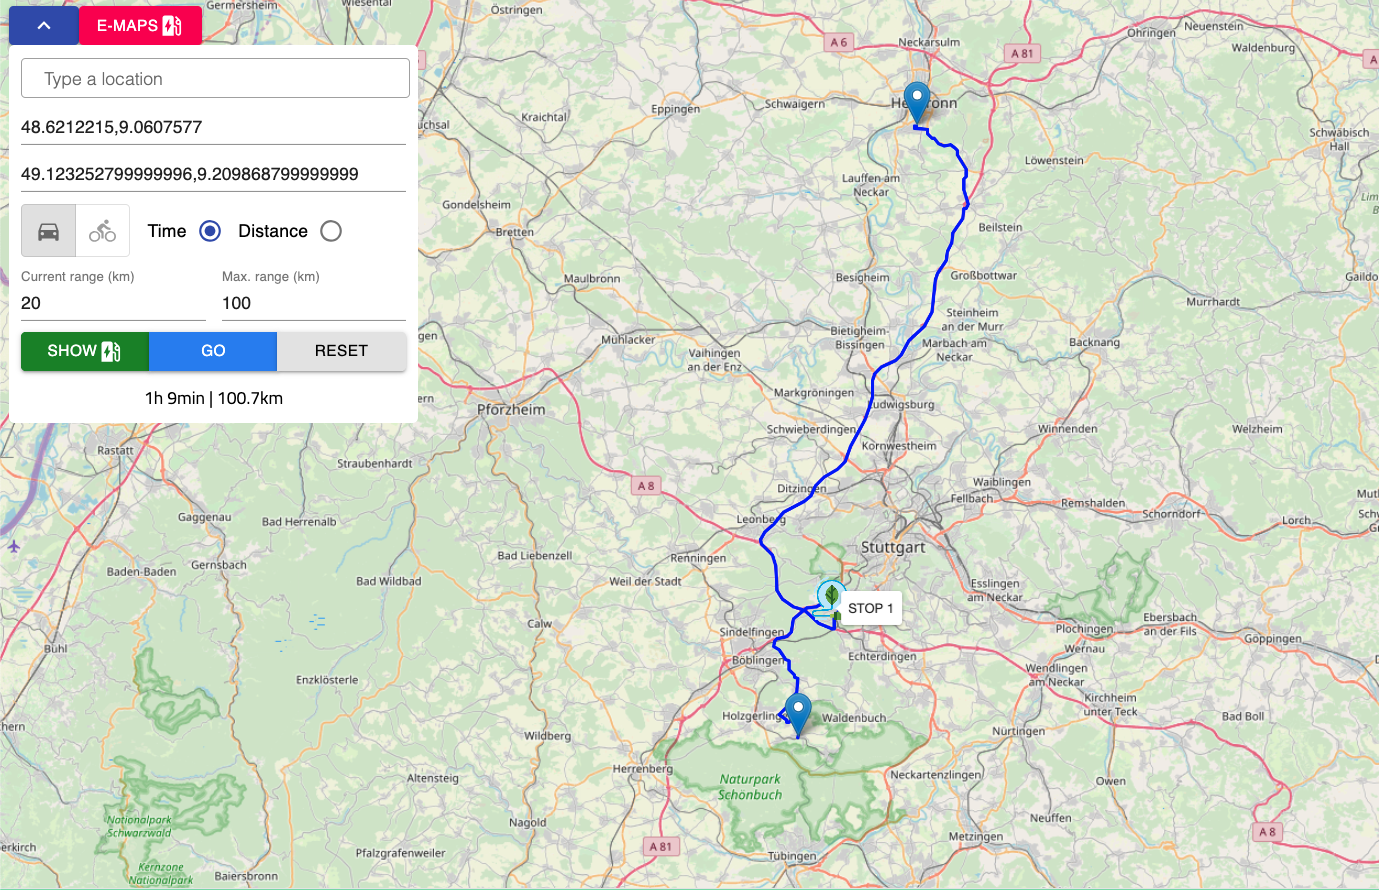
\includegraphics[scale=0.25]{figures/success}
    \caption{Successfully calculation of route with charging stations}
    \label{fig:success}
\end{figure}
\subsection{Further Features}
Another feature of the application is the use of the \textit{Nominatim}\footnote{\url{https://nominatim.openstreetmap.org}} API to allow the user to search for places, cities or Point-Of-Interests (POIs) as seen in Figure \ref{fig:search}.
\begin{figure}[h]
	\centering
	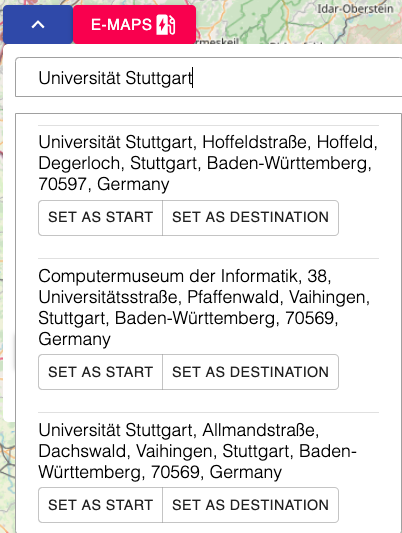
\includegraphics[scale=0.25]{figures/search}
	\caption{Search via Nominatim}
	\label{fig:search}
\end{figure}
Furthermore, it is possible to show (or hide) all charging stations that exist, as seen in Figure \ref{fig:charging}.
These charging stations are, upon request, fetched from the backend via a HTTP GET request and rendered.
\begin{figure}[h]
	\centering
	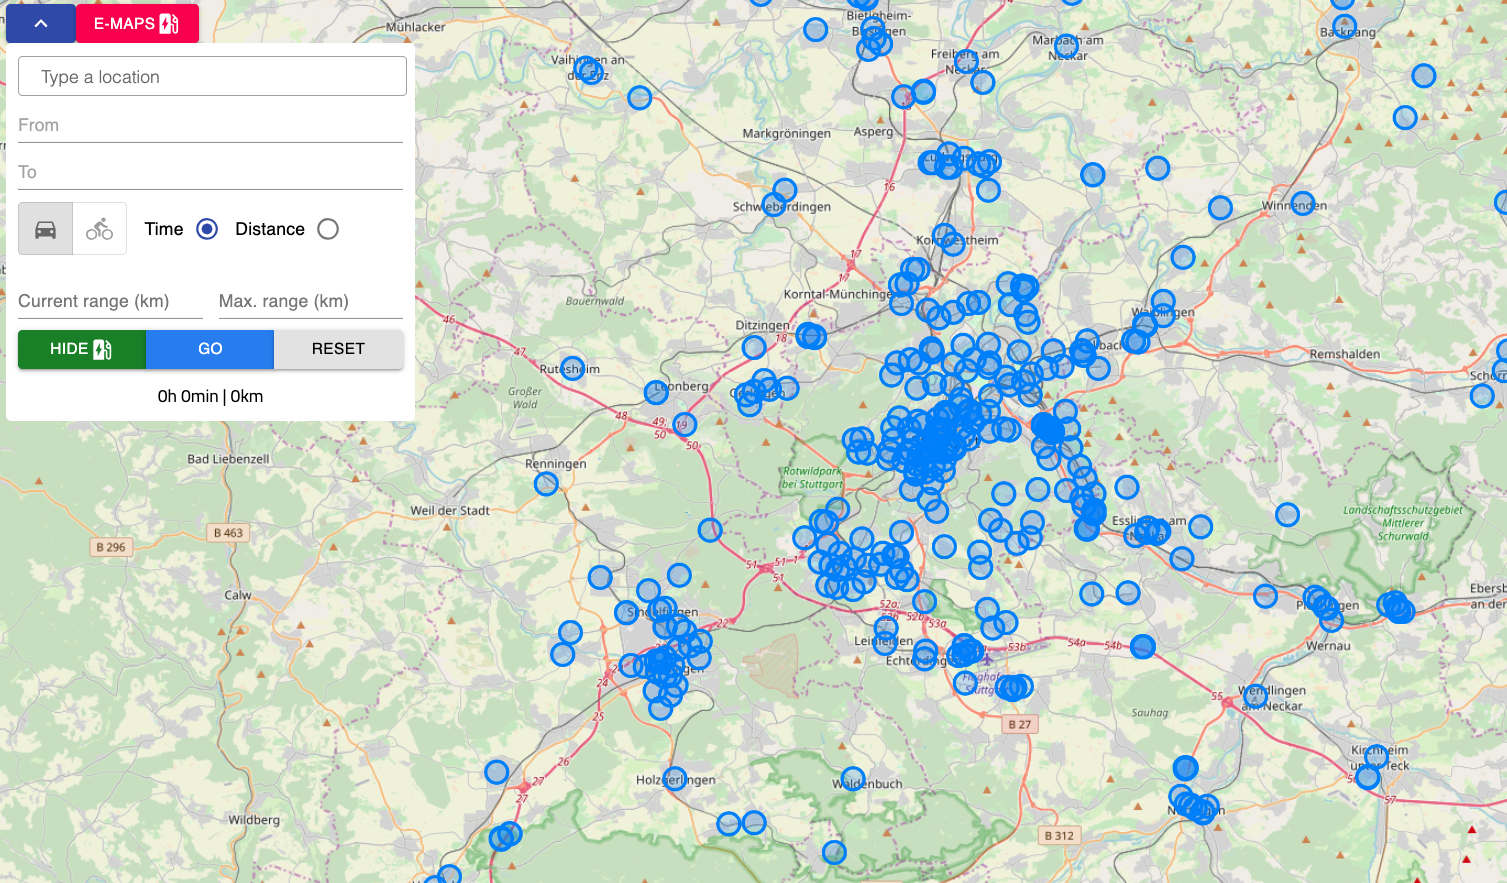
\includegraphics[scale=0.25]{figures/wide}
	\caption{Display all charging stations}
	\label{fig:charging}
\end{figure}
\section{Limitations and Future Work}
Since this project was within the scope of the lecture \textit{Fachpraktikum Algorithms on OpenStreetMap Data} the time spent on the concept and implementation was limited.
Hence, the route calculation with charging stations may not be optimal, as well as determining the charging stations on the route since they follow a rather naive approach.
Furthermore, considering the elevation profile of the road network might help to determine more energy efficient routes for electric vehicles, i.e. routes that go downhill or have a low elevation in general.\par\medskip
For example, Artmeier et al. \cite{Artmeier2010} proposed an extension to general shortest-path algorithms that address the problem of energy-optimal routing by extending a graph with a weight function representing the energy consumption \cite{Artmeier2010}.
To achieve a better routing for electric vehicles in terms of energy efficiency, a similar approach could be implemented on top of this project.\par\medskip
Worley et al. \cite{Worley2012} presented a model that addresses the problem of locating charging stations and calculate routes for electric vehicles based on discrete integer programming optimization and the traditional Vehicle Routing Problem \cite{Worley2012}.
This model could also be used as an orientation to optimize the implementation of choosing a charging stations on the route once required.
\section{Conclusion}
This project demonstrated the use and suitability of OpenStreetMap road network and amenity data to perform route planning for electric vehicles.
The implemented application is a route planner that considers the limited cruising range of electric vehicles, as well as the availability of charging stations along the route.
\bibliographystyle{alpha}
\bibliography{ref}
\end{document}
